\documentclass{llncs}

\usepackage{graphicx}
\usepackage{mwe}
\usepackage{subfig}
\usepackage{amsmath}
\usepackage{amssymb}
\usepackage{rotating}

\begin{document}

\title{Numerical modelling of quantum harmonic oscillator}
\author{Pawel Czyz}

\authorrunning{Pawel Czyz}

\institute{St Hugh's College, University of Oxford}

\maketitle

\begin{abstract}
We present a Python module implementing various ODE solvers, enabling one to do accurate and effective numerical simulations. We investigate it's accuracy investigating a quantum harmonic oscillator in position basis.

\keywords{numerical modelling, Numerov's algorithm, quantum systems, harmonic oscillator}
\end{abstract}

\section{Introduction}
Numerov's method [1] allows one to solve differential equations of kind:

\begin{equation}
\label{eq:num}
	y''(x) = f(x)\cdot y(x)
\end{equation}

Examples of equation (\ref{eq:num}) include classical harmonic oscillator:

\begin{equation}
\label{eq:harm}
	y''(x) = -\omega^2\cdot y(x)
\end{equation}

or one-dimensional, time-independent Schrodinger's equation:
\begin{equation}
\label{eq:quant}
	y''(x)=\frac{2m}{\hbar^2}(E-V(x))\cdot y(x).
\end{equation}

Numerov's iterative method uses an equidistant grid [1,2] $x_n=\delta n$ on which approximates $y_i$ values via equation:

\begin{equation}
\label{eq:iter}
	\left(1-\frac {\delta^2}{12}f_{n+2}\right)y_{n+2}=\left(2+\frac 56\delta^2 f_{n+1}\right)y_{n+1}-\left(1-\frac{\delta^2}{12}f_n\right)y_n,
\end{equation}

where $f_i=f(x_i)$. Equation (\ref{eq:iter}) can be solved for arbitrary $n$ knowing the values $y_0$ and $y_1$.

In practice, second-order differential equations are given Cauchy boundary conditions - $y(0)=y_0$ and $y'(0)=v_0$. Therefore, value $y_1$ is often approximated
using Taylor polynomial:
\begin{equation}
\label{eq:taylor}
y_1=y(\delta)\approx y(0)+ \sum_{n=1}^4 \frac{\delta^n}{n!} y^{(n)}(0).
\end{equation}

Differentiating equation (\ref{eq:num}) and substituting $y''$ for combinations of $y$ and $f$ one gets the fourth-order approximation in terms of $y_0$, $v_0$ and values of different derivatives of $f$, which can be evaluated symbolically or numerically:
\begin{align}
\label{eq:approx}
	y_1 \approx \frac{1}{24} \delta ^4\left(y_0 f''(0)+2 f'(0) v_0+f_0^2 y_0\right) + \\
	+\frac{1}{6} \delta ^3 \left(y_0 f'(0) +f_0 v_0\right)+\frac{1}{2} \delta ^2 f_0
   y_0+\delta  v_0+y_0
\end{align}

\section{Quantum harmonic oscillator}
Schrodinger equation for quadratic potential $V(x)\propto x^2$ can be rewritten in dimensionless form as:
\begin{equation}
  \label{eq:quadr}
  y''(x)=(x^2-E)y(x).
\end{equation}

General theory of differential equations allows one to prove [2, 3] that all the square-integrable solutions are given by:
\begin{equation}
  y_n(x)=H_n(x)\exp \left(-\frac{x^2}2\right),
\end{equation}

where $n$ is a non-negative integer, and $H_n$ is the $n$-th Hermite polynomial. Moreover, such solutions exist only for discrete energies $E_n=2n+1$. We expect that such a solution can be reconstructed using Numerov's method.

We implemented Numerov's method to solve equation (\ref{eq:quadr}) using boundary conditions: $y_0=0,~v_0=1$ ($n$ odd) or $y_0=1,~v_0=0$ ($n$ even) and compared found solutions with analytic one for different energy levels. Figure \ref{fig:oscill}. shows that the method is accurate.

\subsection{Determining oscillator energy levels}
As we are interested in square-integrable solutions, we require $y(x)\to 0$ for $x\to \infty$. Therefore we can determine energy spectrum basing on the behaviour of found function $y$. We implemented a gradient descent optimiser [4] that tried to minimise value $y_E(5)^2$, where $y_E$ is the solution of (\ref{eq:quadr}) for energy value $E$ and with boundary conditions calculated taking $n=[0.5E]$. Table \ref{tab:eigens}. presents found eigenvalues. While found values are close to exact, analytical, values, for $E=1$ there is a small discrepancy. It is due to the small noise at $y_E(5)$.


\begin{figure}
  \centering
  \begin{minipage}{.45\linewidth}
    \centering
    \subfloat[]{\label{fig:oscill:a}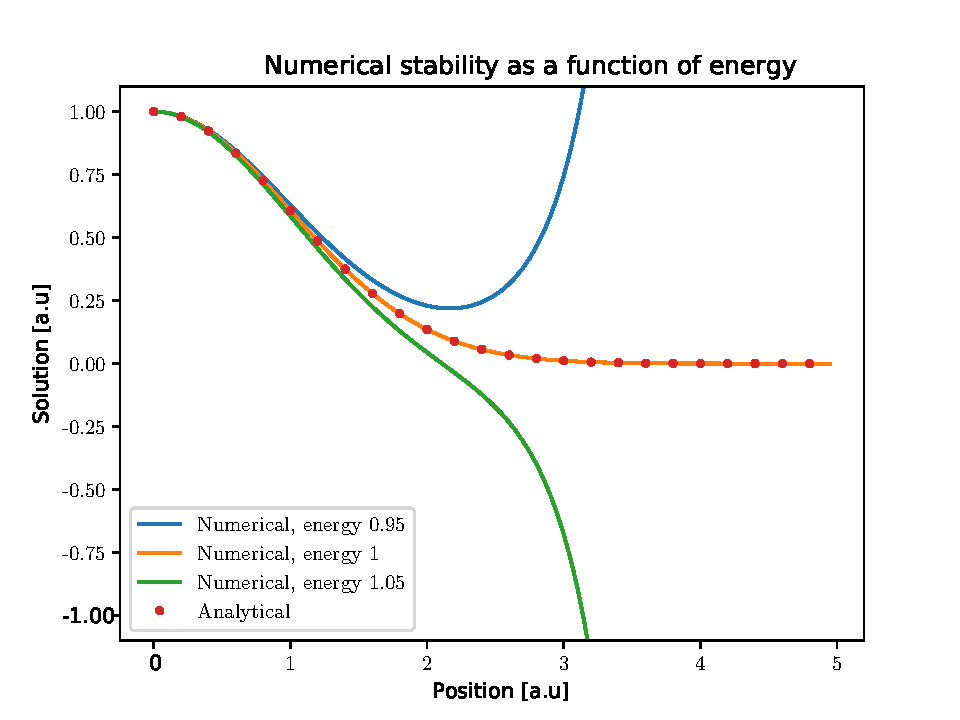
\includegraphics[width=\textwidth]{images/Quantum_oscillator-0}}
  \end{minipage}
  \begin{minipage}{.45\linewidth}
    \centering
    \subfloat[]{\label{fig:oscill:b}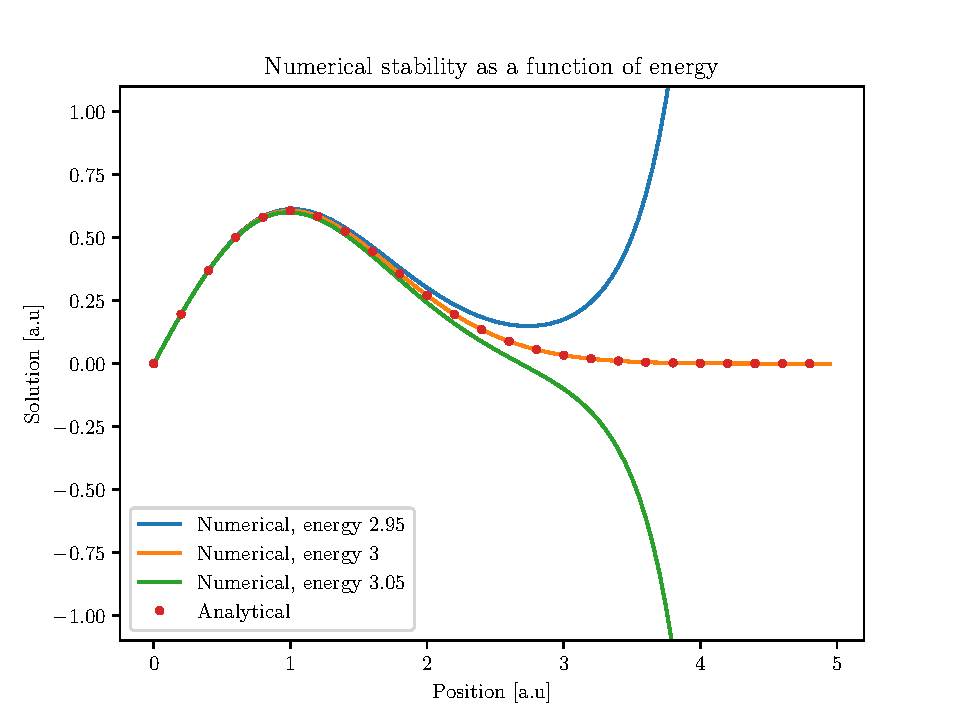
\includegraphics[width=\textwidth]{images/Quantum_oscillator-1}}
  \end{minipage}
  \\
  \begin{minipage}{.45\linewidth}
    \centering
    \subfloat[]{\label{fig:oscill:c}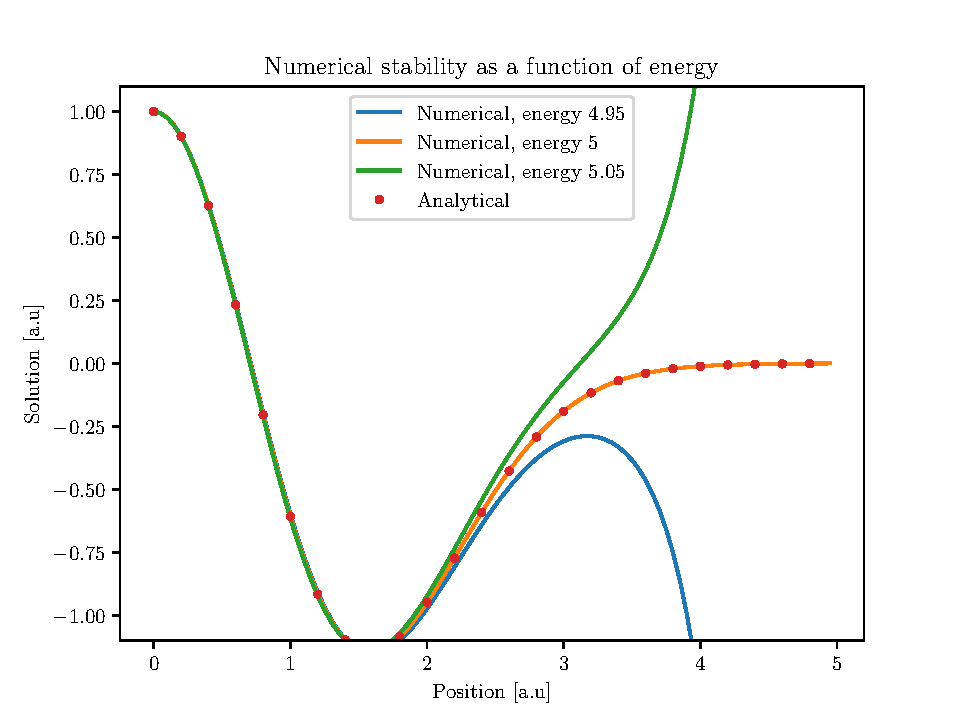
\includegraphics[width=\textwidth]{images/Quantum_oscillator-2}}
  \end{minipage}
  \begin{minipage}{.45\linewidth}
    \centering
    \subfloat[]{\label{fig:oscill:d}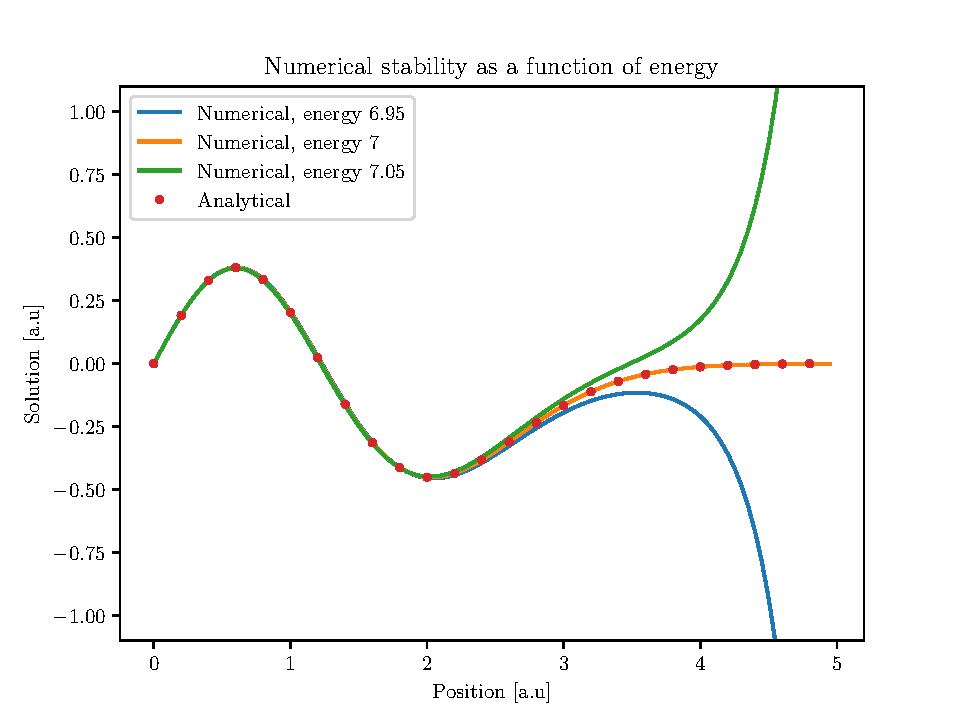
\includegraphics[width=\textwidth]{images/Quantum_oscillator-3}}
  \end{minipage}
  \caption{We compare analytical solution with found numerical solutions for different energy values. We used value $\delta=0.02$ solving equation on the interval $[0,5]$. Different $n$ values were used:
    $n=0$ for \ref{fig:oscill:a}., $n=1$ for \ref{fig:oscill:b}., $n=2$ for \ref{fig:oscill:c}. and $n=3$ for \ref{fig:oscill:d}.}
\label{fig:oscill}
\end{figure}

\begin{figure}
  \centering
  \begin{tabular}{| c | c | c |}
    \hline
    Initial & Found & Exact\\
    \hline
    0.8 & 0.98 & 1 \\
    1.2 & 0.97 & 1 \\
    1.4 & 0.98 & 1 \\
    3.4 & 3.00 & 3 \\
    5.7 & 5.00 & 5 \\
    \hline
  \end{tabular}
  \caption{The table presents found eigenvalues using gradient descent method starting from inaccurate, but close, guessed energy values.}
  \label{tab:eigens}
\end{figure}

\section{Conclusions}

We showed that an oscillator quantised in position basis solved numerically confirms the analytical solution. We found wave-functions corresponding to the different energy levels of the oscillator and confirmed using gradient descent optimiser, that energy spectrum is quantised. Implemented software package can be used to solve other computational physics problems.

\section{References}
\begin{enumerate}
	\item C. Froberg, Introduction to Numerical Analysis, Addison Wesley, 1969.
	\item Joint work, Solutions of Schrodinger's equation by numerical integration, University of Oxford, 2018
	\item R. Schankar, Principles of Quantum Mechanics, Springer, 2008
  \item C. Vogel, Computational Methods for Inverse Problems, SIAM, 2002
\end{enumerate}

\end{document}
